\graphicspath{{chapt_dutch/}{intro/}{monojet/}}

% Header
\renewcommand\evenpagerightmark{{\scshape\small Chapter 5}}
\renewcommand\oddpageleftmark{{\scshape\small The Monojet Analysis}}

\hyphenation{}

\chapter{The Monojet Analysis}
\label{ch:monojet}

As has been described in Chapter~\ref{ch:theory}, there are many searches for dark matter both at 
particle accelerators and elsewhere. At the \ac{LHC}, one very promising channel is the 
monojet search, where the detection of dark matter is done by looking for missing energy in association 
with one or more jets. The dark matter particles are expected to pass through the detector without leaving any signal since they are neutral and only interact very weakly. They can however be detected indirectly as missing energy when they recoil off one or more jets coming from initial state radiation.

First, the event selection and the estimation of the background are described, respectively in Sections~\ref{sec:selection} and \ref{sec:bkgd}. The included systematic uncertainties are described in Section~\ref{sec:syst}. In Section~\ref{sec:results}, the obtained results are shown. The improvements achieved by going from the analysis strategy used in 2015 to the 2016 version are detailed in Section~\ref{sec:improvement}. Finally, the results are interpreted in terms of the considered dark matter models in Section~\ref{sec:interpretation}.

% {\color{red}models in theory chapter?\\
% MET: add in chapter 3: + type I corrections from jets + corrections in simulation as well to match data)\\
% b-tagging: add in chapter 3}\\
% {\color{red} add in chapter 3: loose jet ID, pileup jet ID}.

\section{Event selection}
\label{sec:selection}

In order to select events that have the Monojet signature illustrated in Figure~\ref{fig:monojet_diagram}, the trigger requires either $E_T^{miss} > 90$~GeV, where $E_T^{miss}$ is the magnitude of the negative vectorial sum of the $p_T$ of all particles at trigger level, or $H_T^ {miss} > 90$ ~GeV, where $H_T^{miss}$ is calculated as the magnitude of the negative vectorial sum of the momenta of all jets with $p_T > 20$~GeV. Muons are not taken into account to compute $E_T^{miss}$ and $H_T^{miss}$, so that the same trigger can be used to select the events for the muon control regions used for the background prediction. The trigger efficiency is above 98\% for events passing the analysis selection described below.

\begin{figure}[ht]
  \centering
 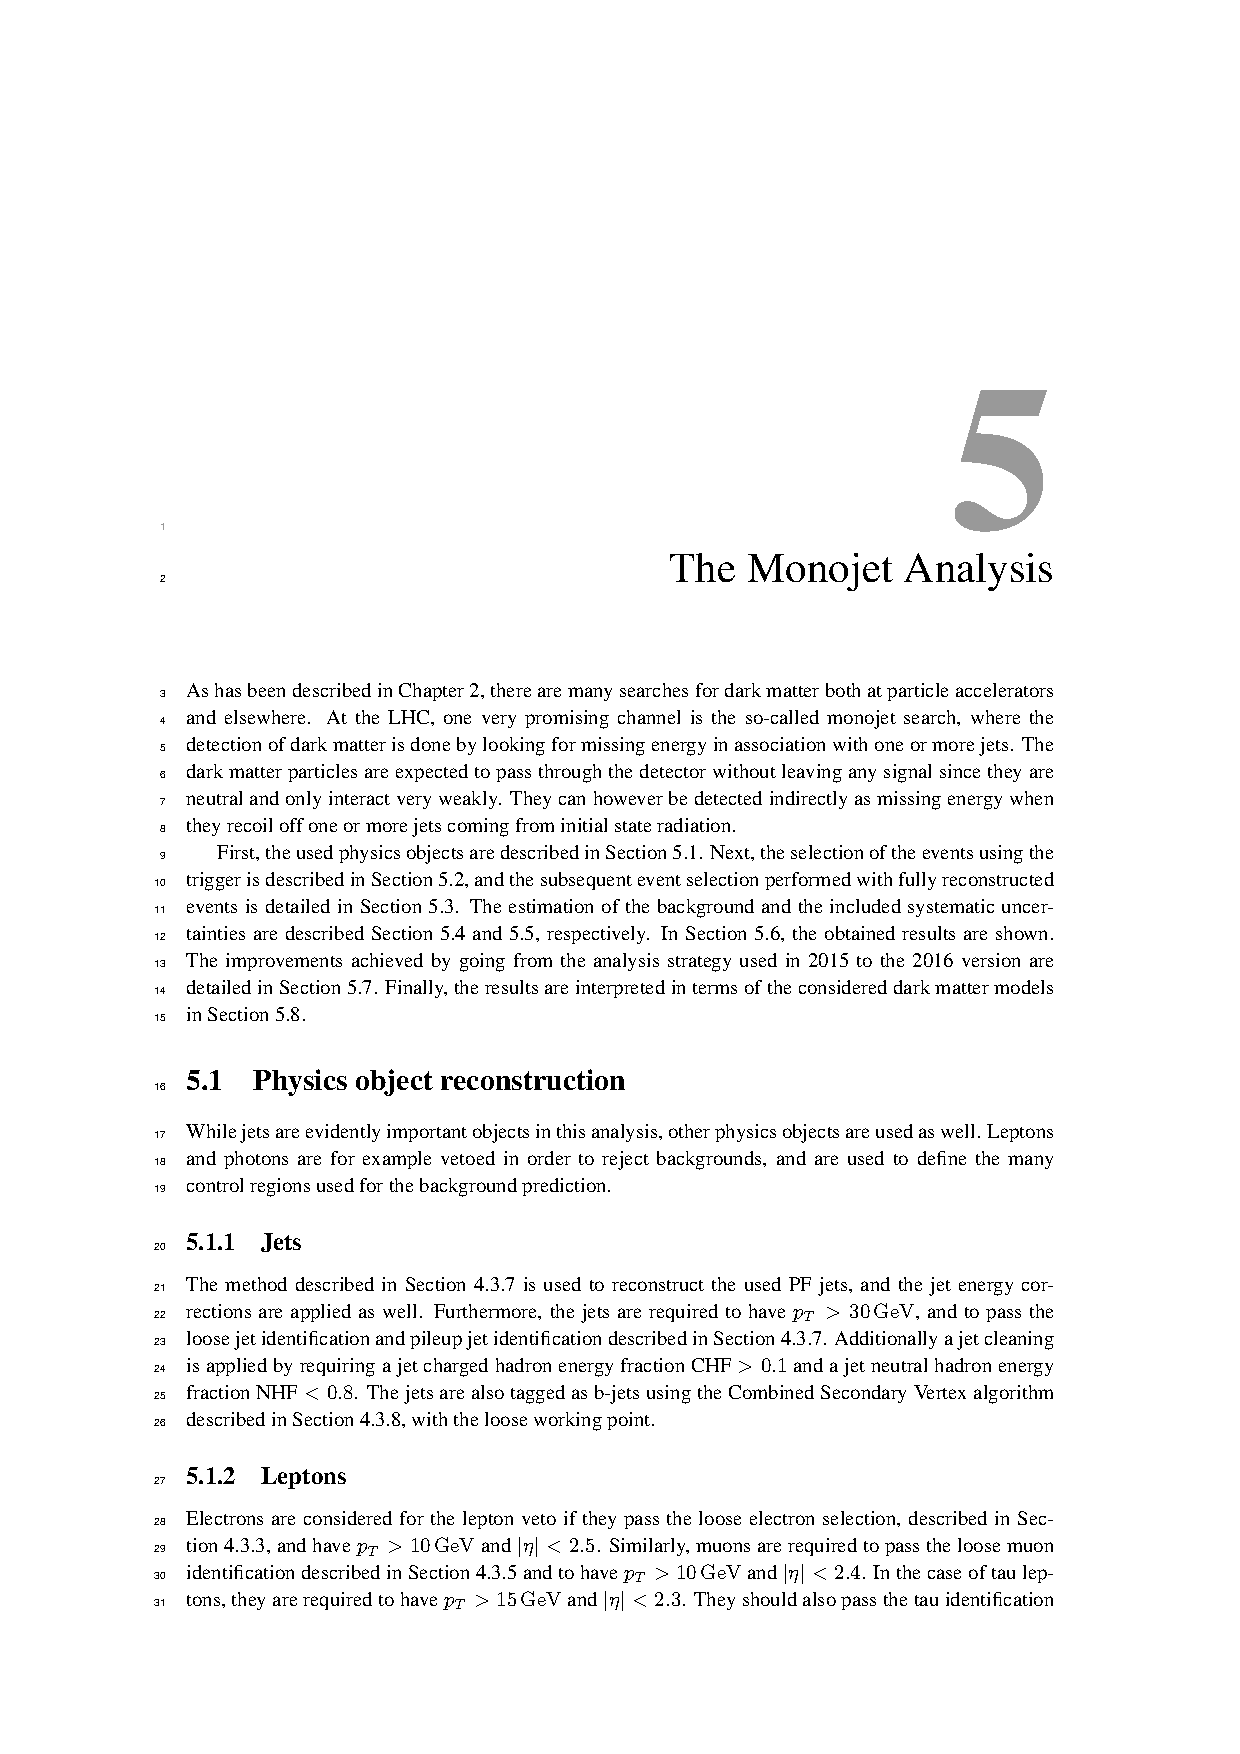
\includegraphics[width=.4\textwidth]{monojet.png} 
 \caption{Illustration of dark matter production in the monojet final state.}
 \label{fig:monojet_diagram}
\end{figure}

Once the events have been fully reconstructed and the jets in the event have been corrected as described in Section~\ref{sec:jet_reconstruction}, an event selection is applied by requiring the missing transverse energy $E_T^{miss}$ defined in Section~\ref{sec:MET} to be larger than 200~GeV in order to be consistent with the trigger turn-on. Additionally, the leading jet is required to have $p_T > 100$~GeV, $|\eta| < 2.5$, and to pass the loose jet identification and pileup jet identification described in Section~\ref{sec:jet_reconstruction}, as well as the jet cleaning.  The jet cleaning is done by requiring a jet charged hadron energy fraction CHF $> 0.1$ and a jet neutral hadron energy fraction NHF $< 0.8$. The same requirements are applied for the remaining jets to be taken into account, except for the $p_T$ threshold which is at 30~GeV in this case. A cut on the difference in azimuthal angle between the $E_T^{miss}$ and the first four leading jets of $\Delta\phi(jet, E_T^{miss}) > 0.5$ is also applied to suppress the QCD background from mismeasurements of jet momentum or detector noise. The events are further cleaned by applying quality filters to remove events with badly reconstructed missing transverse energy. Finally, events containing a lepton, a photon, or a b-jet are vetoed as well.

The leptons are vetoed to suppress the electroweak backgrounds, such as $W(lv)$ + jets and semileptonic diboson decays. Electrons (muons) are considered for the veto if they pass the loose selection and have $p_T > 10$~GeV and $|\eta| < 2.5 (2.4)$. In the case of tau leptons, they are required to have $p_T > 15$~GeV and $|\eta| < 2.3$. They should also pass the tau identification criteria, which require a jet with an identified subset of particles with a mass consistent with the decay products of a hadronic tau and which are isolated with a pileup corrected isolation cut requiring less than 5~GeV of energy deposits within a radial cone of $\Delta R < 0.3$. Photons are required to have $p_T > 15$~GeV, $|\eta| < 2.5$, and to pass the {\color{red}loose identification} criteria. The photon veto is added to suppress the $Z(\nu\nu)$ + photon + jets and $W(l\nu)$ + photon + jets background processes, and to ensure there is no overlap with a similar dark matter search which investigates the final state consisting of missing energy and a photon. This rejects less than 1\% of the signal. Finally, the b-jet veto reduces the top background by a factor 3 and only reduces the signal by 5 to 10\%, depending on the type and mass of the mediator. The b-jets are tagged with the CombinedSecondaryVertexv2 algorithm described in Section~\ref{sec:btagging}, using {\color{red} working point? $> 0.89$}

\section{Background estimation}
\label{sec:bkgd}

% {\color{red} muons: muon veto to suppress electroweak bkgds
% pt > 10, eta < 2.4, loose selection:
% muons for control regions: global, pf, global track chi2 < 10, global track fit includes >= 1 muon chamber hit, muon segments in >= 2 muon stations, transverse impact parameter wrt PV < 2mm, longitudinal impact parameter < 5mm, >= 1 pix hit, > 8 trk layers hit, hits in >= 5 tracker layers, delta beta < 0.12
% 
% electrons: electron veto to suppress electroweak bkgds
% pt > 10, eta < 2.5,  loose selection(table 10)
% electrons in control region: tight selection (table 11)
% 
% photons in control region to estimate Znunu bkgd: tighter selection table 13
% < 1\% rejection of signal
% For muons and
% electrons this reduces the influence of large brehmstrahlung, further minimizing anomalous
% effects that would modify the recoil.
% 
% photon purity (2 methods):
% 
% lepton and photon eff: 2 methods}

The dominant background comes from $Z$ + jet events where the $Z$ boson decays to two neutrinos. This produces the same signature of jets with missing energy as the signal, and results in an irreducible background. The second largest background consists of $W$ + jets events with a leptonically decaying $W$ boson. This background is already suppressed by the lepton veto, but a fraction of these events remain when the lepton is either not identified or outside of the detector acceptance. The remaining background events come from top quark decays, which are suppressed by the b-jet veto, semileptonic diboson ($WW$, $WZ$, and $ZZ$) decays, and QCD multijet events. The two main background contributions are estimated from five control regions in data consisting of dimuon, dielectron, single muon, single electron, and photon + jets events. The $E_T^{miss}$ in these control regions is redefined in order to imitate the $E_T^{miss}$ shape in the signal region. This hadronic recoil $U$ is obtained by removing the leptons or the photon from the $E_T^{miss}$ computation. The contributions from top quark decays and semileptonic diboson decays are estimated using simulated samples, while the QCD multijet background is estimated using a data-driven approach.

\subsection{The \boldmath$Z$ and \boldmath$W$ background estimation}

The yield of $Z(\nu\nu)$ and $W(l\nu)$ + jets events in the signal region is estimated from five control regions by using the ratio between data and MC in the control region, per bin of the recoil distribution. For the prediction using $Z\rightarrow \mu\mu$ events in the dimuon control region for example, the predicted yield of $Z\rightarrow\nu\nu$ events is given by
\begin{align}
 N_{Z(\nu\nu)} &= \frac{N_{Z(\mu\mu)}^{data}}{N_{Z(\mu\mu)}^{MC}}\ N_{Z(\nu\nu)}^{MC}\\
 &= \frac{N_{\mu\mu}^{data} - N_{Bkgd}}{N_{Z(\mu\mu)}^{MC}}\ N_{Z(\nu\nu)}^{MC} \\
 &= \frac{N_{\mu\mu}^{data} - N_{Bkgd}}{N_{Z(\mu\mu)}^{MC}}\ R_{Z(\mu\mu)\rightarrow Z(\nu\nu)}\ N_{Z(\mu\mu)}^{MC}
\end{align}
The transfer factors, denoted by $R$, are derived from simulation and take into account the impact of lepton acceptance and efficiency, as well as the additional $E_T^{miss}$ requirement for the single electron control region. They also include the difference in branching ratio and the relation between the differential cross sections of the photon, $W$, and $Z$ boson production as a function of the boson $p_T$. The transfer factors are computed as a function of the recoil, and are shown for the five different control regions in Figure~\ref{fig:TF}. Furthermore, the $Z/W$ ratio shown in the bottom right plot of Figure~\ref{fig:TF} provides an additional constraint since the single lepton control regions are also used to  estimate the $Z(\nu\nu)$ + jets background.

\begin{figure}[h!]
  \centering
 \vspace{.3cm}
 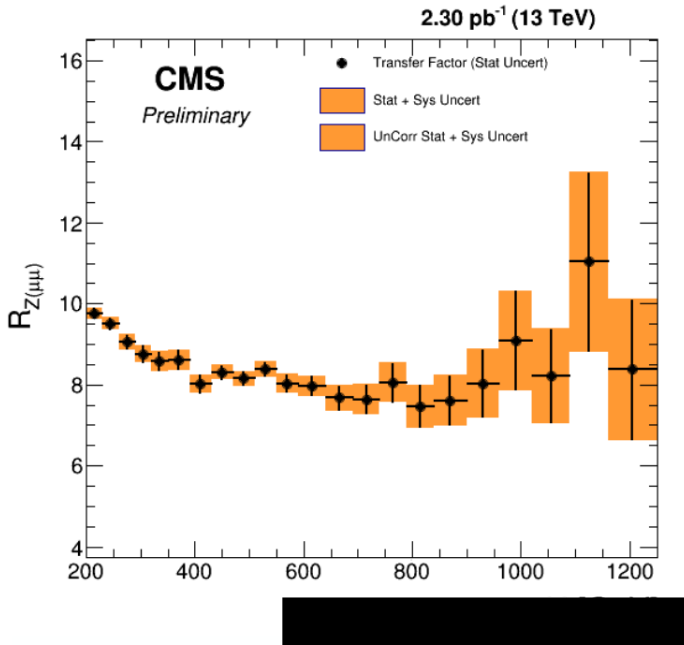
\includegraphics[width=.49\textwidth]{dimuon_TF.png} 
 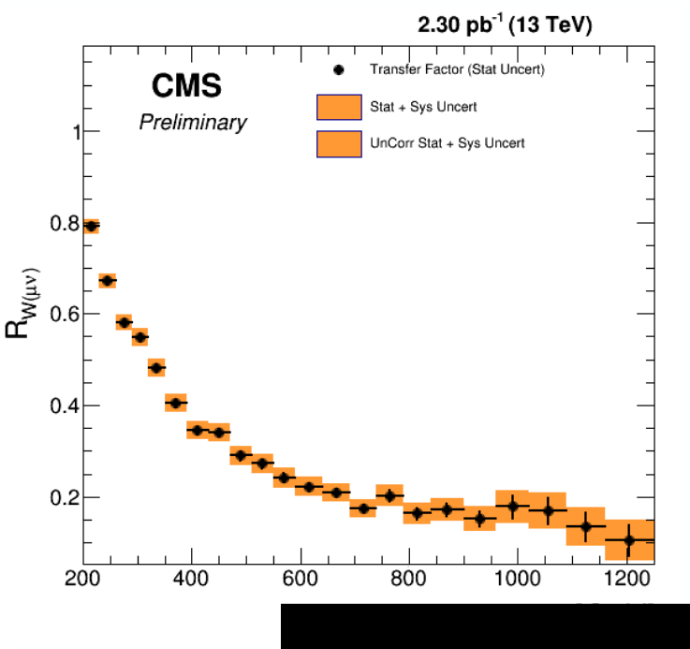
\includegraphics[width=.5\textwidth]{single_muon_TF.png} \\
 \vspace{.4cm}
 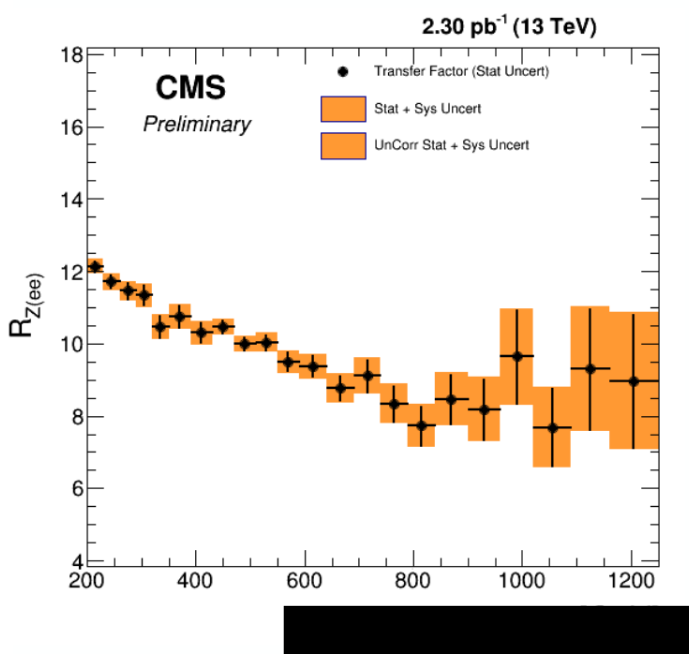
\includegraphics[width=.49\textwidth]{dielectron_TF.png} 
 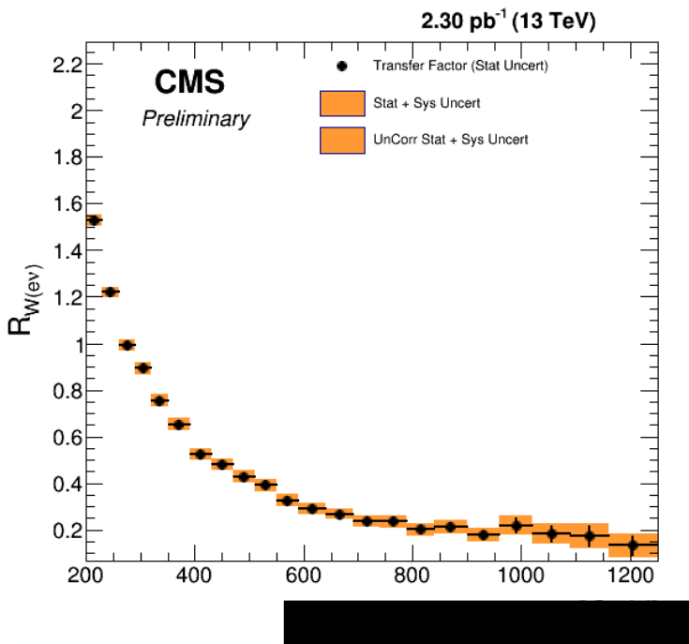
\includegraphics[width=.5\textwidth]{single_electron_TF.png} \\
 \vspace{.2cm}
 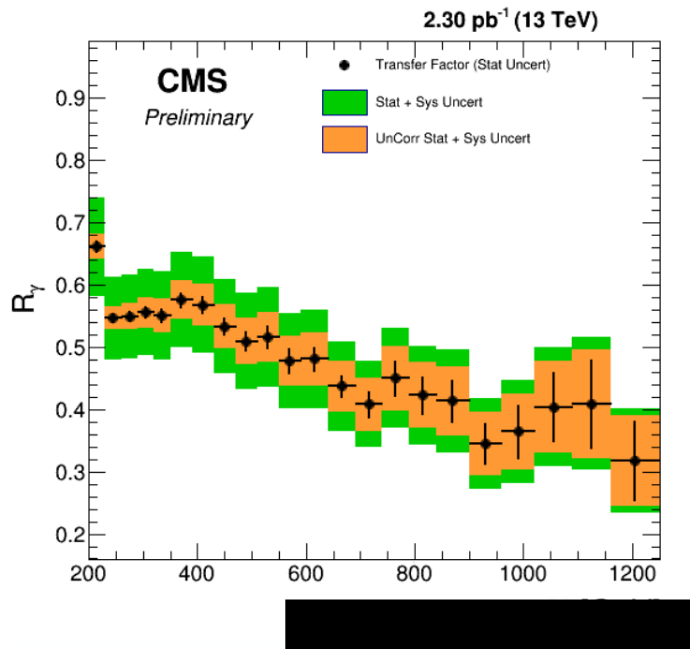
\includegraphics[width=.49\textwidth]{gamma_TF.png} 
 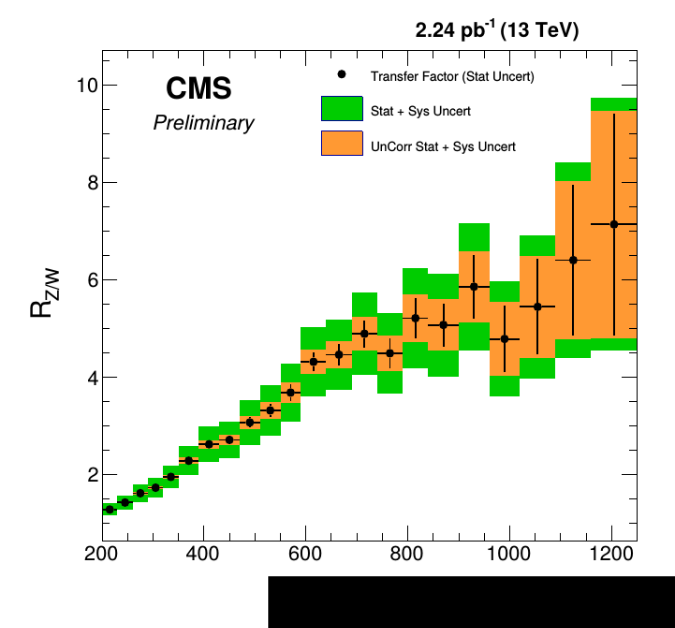
\includegraphics[width=.5\textwidth]{ZW_ratio.png} 
 \caption{Transfer factors for the dimuon (top left), single muon (top right), dielectron (middle left), single electron (middle right), and photon + jets (bottom left) control regions. The ratio of the $Z$ and $W$ transfer factors is shown in the bottom right plot.}
 \label{fig:TF}
\end{figure}

The simulated samples used for the background estimation are generated at leading order (LO) using the \textsc{Madgraph} generator, and corrected to next-to-leading order (NLO). These corrections introduce an additional systematic uncertainty, but are crucial in order correctly represent the data, since the simulation is approximately 40\% higher than the data when using only LO calculations. The NLO QCD k-factors are derived from samples generated at NLO with \textsc{MadGraph5\_}a\textsc{MC@NLO}, while the electroweak k-factors are obtained from theoretical calculations~\cite{Kuhn:2005gv, Kallweit:2015fta, Kallweit:2014xda, Kallweit:2015dum}. The differential cross section as a function of the boson $p_T$ is shown in Figure~\ref{fig:kfactors} for photon, $W$,and $Z$ production, and the obtained k-factors are displayed in the ratio plots. More details on the different control regions are given in the following description.

\begin{figure}[ht]
  \centering
 \includegraphics[width=.49\textwidth]{Z_EWK_kfactor.pdf} 
 \includegraphics[width=.49\textwidth]{W_EWK_kfactor.pdf} \\
 \includegraphics[width=.49\textwidth]{gamma_EWK_kfactor.pdf} 
 \caption{ The differential cross section as a function of the boson $p_T$ for photon, $W$,and $Z$ production, with the resulting k-factors in the ratio plots.}
 \label{fig:kfactors}
\end{figure}

\begin{itemize}
 \item[] \textbf{Dimuon control region}\\ The traditional control region for the $Z$ boson background is the dimuon control region. This region is dominated by $Z\rightarrow\mu\mu$ events, which are very similar to the $Z(\nu\nu)$ + jets background events, the only difference being the decay mode. The production mode and kinematics in the control region are very similar, as well as the acceptance. However, the branching ratio of the $Z$ boson into two muons is 6 times smaller than the branching ratio to two neutrinos. As a result, the dimuon control region contains about 10 times less $Z$ boson events than the signal region. In order to improve this statistical limitation, other control regions have been added as well.

In the dimuon control region the events are selected using the monojet triggers and applying the same requirements as described in Section~\ref{sec:selection} for the signal region, using the recoil instead of the missing transverse energy, except for the muon veto. Additionally, exactly two muons with opposite charge and with $p_T > 10$~GeV should be identified using the loose identification {\color{red}described in Section ? (or listed in Table ?)}. At least one muon is required to have $p_T > 20$~GeV and to pass the tight selection requirements {\color{red}described in Section ? (or listed in Table ?)}, and the leading muon should also have a transverse momentum large than 20~GeV. Finally, the dimuon mass should be between 60 and 120~GeV, corresponding to the $Z$ boson mass.

\item[] \textbf{Single muon control region}\\ In order to model the second largest background, coming from $W(l\nu)$ + jets events, a single muon control region is typically used. This control region is in addition also used to constrain the $Z(\nu\nu)$ + jets background. The events in the single muon control region are required to pass the monojet triggers and event selection replacing the $E_T^{miss}$ by the recoil obtained by removing the muon, except for the muon veto. One muon should then pass the {\color{red} tight selection} requirements and have $p_T > 20$~GeV.

\item[] \textbf{Dielectron and single electron control region}\\ The dielectron and single electron control regions are completely analogous to the dimuon and single muon control regions, respectively. These events are required to pass the single electron triggers. Similarly to the dimuon control region, the events in the dielectron control region are required to pass the monojet selection, except for the electron veto. Instead, exactly two electrons with $p_T > 10$~GeV are required to pass the loose identification {\color{red}described in Section ? (or listed in Table ?)} In addition, at least one electron should pass the tight selection requirements and have $p_T > 20$~GeV. Finally, the dielectron mass should be between 60 and 120~GeV, in order to be consistent with a $W$ boson decay. {\color{red}transfer factor last bin due to isolation in trigger}. The dielectron control region is used to constrain the $Z\rightarrow\nu\nu$ background while the single electron control region is used to constrain the $W(l\nu)$ + jets background. In the single electron control region, the events are required to have one electron passing the tight selection requirements and having $p_T > 20$~GeV, analogously to the single muon control region. In this region, a large amount of QCD background is present. In order to reject most of those events, an additional cut on the $E_T^{miss}$, which includes the single electron, is added at 50~GeV. This reduces the QCD background by an order of magnitude.

\item[] \textbf{Photon + jets control region}\\Due to its large yield, photon + jets control region provides the dominant constraint on the high-$p_T$ part of the $Z(\nu\nu)$ + jets background. The selection of these events is done using the single photon triggers and applying the monojet selection, except for the photon veto. One photon is then required to pass the tight identification {\color{red}described in Section ? (or listed in Table ?)} and to have $p_T > 175$~GeV and $|\eta| < 1.4442$. Events with more than one photon passing the loose identification requirements {\color{red}described in Section ? (or listed in Table ?)} are rejected.
\end{itemize}

\subsection{The QCD background estimation}

\section{Systematic uncertainties}
\label{sec:syst}

For the main backgrounds, multiple systematic uncertainties on the transfer factors are taken into account. Experimental uncertainties are added for the muon efficiency, the electron efficiency, the lepton veto, the photon efficiency, and the photon purity in the photon + jets sample. 

Uncertainties are also added from theory, to take into account variations of the factorization and renormalization scales, PDF uncertainties, and the NLO electroweak corrections. The former 3 uncertainties are shown in Figure~\ref{fig:kfactors_unc} for the $Z$ + jets, $W$ + jets, and photon + jets samples. The  uncertainties are then propagated to the transfer factors, and are displayed in Figure~\ref{fig:transfer_factors_unc}. To evaluate the PDF uncertainty, the samples are reweighted with event-by-event scale factors representing the shift in the kinematic distributions from variations in the PDF. The transfer factors are then produced for each variation, and the RMS of the variation is taken as PDF uncertainty. Similarly, the renormalization and factorization scales are varied up and down by a factor 2, and the uncertainties are derived from the resulting transfer factors. For the electroweak corrections, the full correction is taken as an uncertainty.

\begin{figure}[ht]
  \centering
 \includegraphics[width=.49\textwidth]{Z_uncertainties_smooth.pdf} 
 \includegraphics[width=.49\textwidth]{W_uncertainties_smooth_new.pdf} \\
 \includegraphics[width=.49\textwidth]{gamma_uncertainties_smooth.pdf} 
 \caption{The PDF, renormalization, and factorization scale uncertainties for the $Z$ + jets (top left), $W$ + jets (top right), and photon + jets (bottom) samples. The uncertainties from the renormalization and factorization scales are obtained by separately varying them up and down by a factor 2.}
 \label{fig:kfactors_unc}
\end{figure}

\begin{figure}[ht]
  \centering
 \includegraphics[width=.49\textwidth]{fig.pdf} 
 \includegraphics[width=.49\textwidth]{fig.pdf}
 \caption{.}
 \label{fig:transfer_factors_unc}
\end{figure}

\section{Results}
\label{sec:results}

The results are extracted by performing a binned fit to the missing energy spectrum, fitting simultaneously over the five control regions and the signal region. 

\section{Improvement going from the 2015 to 2016 analysis}
\label{sec:improvement}

One of the improvements that were added to the monojet analysis is the use of MC samples generated at leading order for the estimation of the main backgrounds. This was possible by generating samples that are binned in photon, $Z$, or $W$ boson $p_T$. As a result, no k-factors need to be applied to samples generated at LO and no additional systematic uncertainties need to be introduced for this.

\section{Interpretation}
\label{sec:interpretation}

\clearpage{\pagestyle{empty}\cleardoublepage}
